\index{KIWI images!maintenance|(}
\chapter{Maintenance of Operating System Images}
\label{chapter:maintain}
\minitoc

Creating an image often results in an appliance solution for a
customer and gives you the freedom of a working solution at that
time. But software develops and you don't want your solution to
become outdated. Because of this together with an image people always
should think of \textbf{image-maintenance}. The following paragraph
just reflects ideas how to maintain images created by kiwi:

\begin{figure}[h]
\centering
\includegraphics[scale=0.5]{pictures/maintain.eps}
\caption{Image maintenance scenarios}
\label{fig:maintenance}
\end{figure}

The picture above shows two possible scenarios which requires an
image to become updated. The first reason for updating an image
are changes to the software, for example a new kernel should be
used. If this change doesn't require additional software or changes
in the configuration the update can be done by kiwi itself using
its \textbf{upgrade} option. In combination with \textbf{upgrade}
kiwi allows to add an additional repository which may be needed if
the updated software is not part of the original repository. An
important thing to know is that this additional repository is \textbf{not}
stored into the original config.xml file of the image description.

Another reason for updating an image beside software updates are
configuration changes or enhancements, for example an image should
have replaced its browser with another better browser or a new service
like apache should be enabled. In principal it's possible to do all
those changes manually within the physical extend but concerning
maintenance this would be a nightmare. Why, because it will leave the
system in an unversioned condition. Nobody knows what has changed
since the very first preparation of this image. So in short
\textbf{dont't modify physical extends manually}. Changes to the image
configuration should be done within the image description. The
image description itself should be part of a versioning system like
subversion. All changes can be tracked down then and maybe more
important can be assigned to product tags and branches. As a consequence
an image must be prepared from scratch and the old physical extend
could be removed.
